\documentclass[UTF8]{report}
\usepackage[margin=0.5in]{geometry}
\usepackage{graphicx}
\usepackage{xetexko}

\title{%
    <컴퓨터프로그래밍 3> 실습 보고서 \\
    \large [제 10 주] 후위연산식계산기 1-1}
\author{201704150 허강준}
\date{\today}

\begin{document}
    \maketitle
    \tableofcontents

    \chapter{프로그램 설명서}
        본 보고서에서는 스택을 정의 및 구현하고 이를 응용하여 후위연산식을 계산하는 프로그램에 대해 기술한다.

        \section{프로그램의 전체 설계 구조 (MVC 등)}

            \paragraph{%
                \normalfont 본 스택 응용 프로그램은 크게 프로그램의 제어를 담당하는 Controller인 \texttt{app\_controller}, 입/출력을 담당하는 View인 \texttt{app\_view}, 그리고 스택을 정의하고 구현하는 \texttt{stack} 모델을 정의한다. \texttt{stack}모델은 이전에 계속 사용된 \texttt{vector} Type의 Wrapper 클래스이다. 여기에 더불어, 후위연산식 계산을 처리하기 위한 \texttt{postfix} Type을 추가로 정의한다.
            }

        \section{함수 설명서}

            \paragraph{\texttt{VECTOR(type)}}
            \paragraph{%
                \normalfont C++의 Standard Template Library에 정의된 Container Template Type인 \texttt{vector}를 일부 구현하였다. 구현된 메서드는 \texttt{new},  \texttt{delete}, \texttt{at}, \texttt{front}, \texttt{back}, \texttt{data}, \texttt{empty}, \texttt{size}, \texttt{max\_size}, \texttt{clear}, \texttt{insert}, \texttt{erase}, \texttt{push\_back}, \texttt{pop\_back}, \texttt{swap} 이다.
            }

            \paragraph{\texttt{stack}}
            \paragraph{%
                \normalfont \texttt{VECTOR(char) 의 type alias}
            }

            \paragraph{\texttt{app\_controller\_create}}
            \paragraph{\texttt{app\_controller\_run}}
            \paragraph{\texttt{app\_controller\_exit}}
            \paragraph{\texttt{app\_controller\_get\_result}}
            \paragraph{\texttt{app\_controller\_delete}}
            \paragraph{%
                \normalfont \texttt{app\_controller} 주요 공개함수들로 프로그램의 제어에 관여한다.
            }


            \paragraph{\texttt{getchar\_direct}}
            \paragraph{\texttt{appview\_in\_char\_directly\_from\_keyboard}}
            \paragraph{%
                \normalfont 키보드로부터 직접 키 입력을 받아온다. Control Sequence가 아닌 경우 echo도 같이 수행한다.
            }



            \paragraph{\texttt{appview\_out\_top\_of\_stack}}
            \paragraph{\texttt{appview\_out\_bottom\_of\_stack}}
            \paragraph{%
                \normalfont 스택 전체 출력시 처음과 끝이 각각 bottom, top임을 출력한다.
            }

            \paragraph{\texttt{appview\_out\_element}}
            \paragraph{%
                \normalfont 지정된 요소 하나를 출력한다.
            }
            
            \paragraph{\texttt{appview\_out\_new\_line}}
            \paragraph{%
                \normalfont 화면상에서 개행한다.
            }

            \paragraph{\texttt{appview\_out\_start\_program}}
            \paragraph{\texttt{appview\_out\_end\_program}}
            \paragraph{%
                \normalfont 프로그램의 시작과 끝을 알리는 메세지를 출력한다.
            }

            \paragraph{\texttt{stack\_new}}
            \paragraph{\texttt{stack\_delete}}
            \paragraph{%
                \normalfont 스택 객체 생성 및 삭제 함수
            }

            \paragraph{\texttt{stack\_push}}
            \paragraph{\texttt{stack\_pop}}
            \paragraph{%
                \normalfont 스택의 push, pop 동작 구현
            }

            \paragraph{\texttt{stack\_peek}}
            \paragraph{\texttt{stack\_at}}
            \paragraph{%
                \normalfont 스택의 peek, at 동작 구현
            }

            \paragraph{\texttt{stack\_size}}
            \paragraph{%
                \normalfont 스택에 저장된 요소의 크기를 반환한다.
            }

            \paragraph{\texttt{stack\_full}}
            \paragraph{\texttt{stack\_empty}}
            \paragraph{%
                \normalfont 스택이 꽉 찼는지, 비었는지 여부를 반환한다.
            }

        \section{종합 설명서}

            \paragraph{%
                \normalfont 본 프로그램은 키보드로부터 직접 \texttt{stack}은 이전에 매크로로 구현한 제너릭 타입인 \texttt{VECTOR}에 대하여 \texttt{char}형을 다루게 끔 한 후 \texttt{typedef} 한 것이다. 그러나 스택으로서 더욱 특화되도록 일부 메서드를 추가 구현해 주었다.
            }

    \chapter{프로그램 장단점/특이점 분석}
            \section{생각해 볼 점: \texttt{char*} 와 String}

    \chapter{실행 결과 분석}
        \section{실행 결과}
        \paragraph{%
            \begin{figure}[!htb]
                \centering
                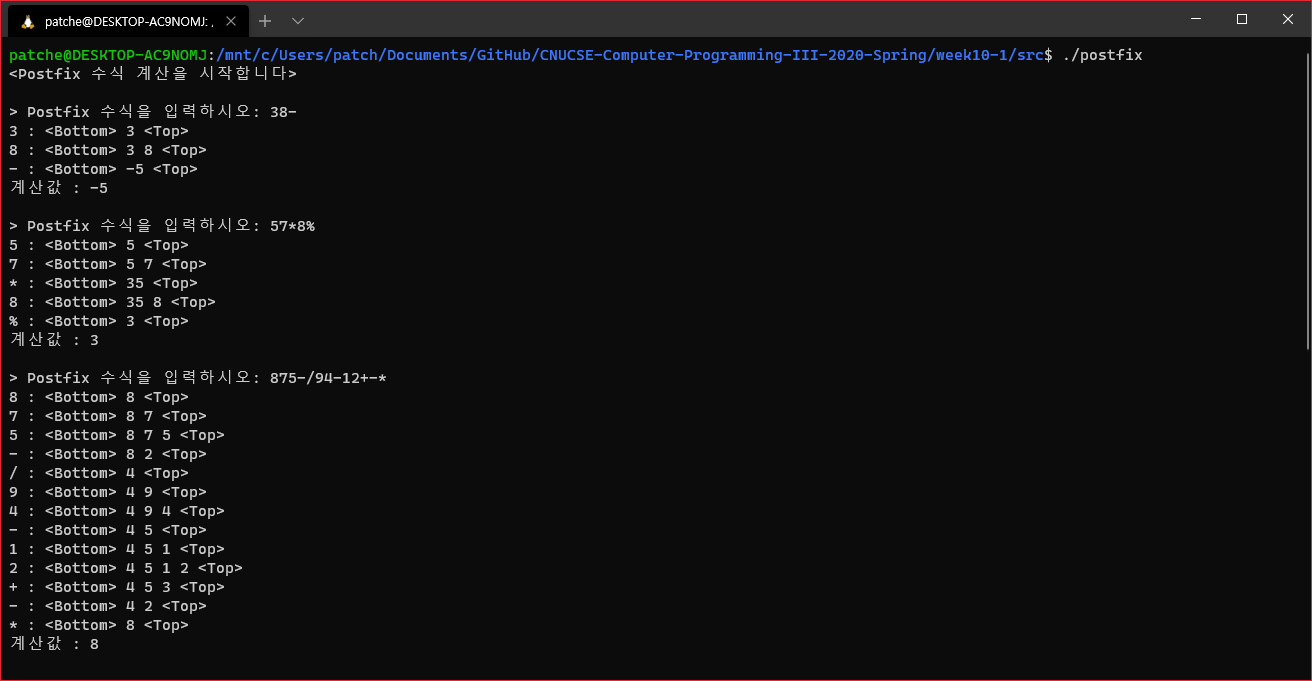
\includegraphics[width=\textwidth]{result_1.png}
                \caption{자료 제시 입력 실행결과 1}
                \label{}
            \end{figure}
            \begin{figure}[!htb]
                \centering
                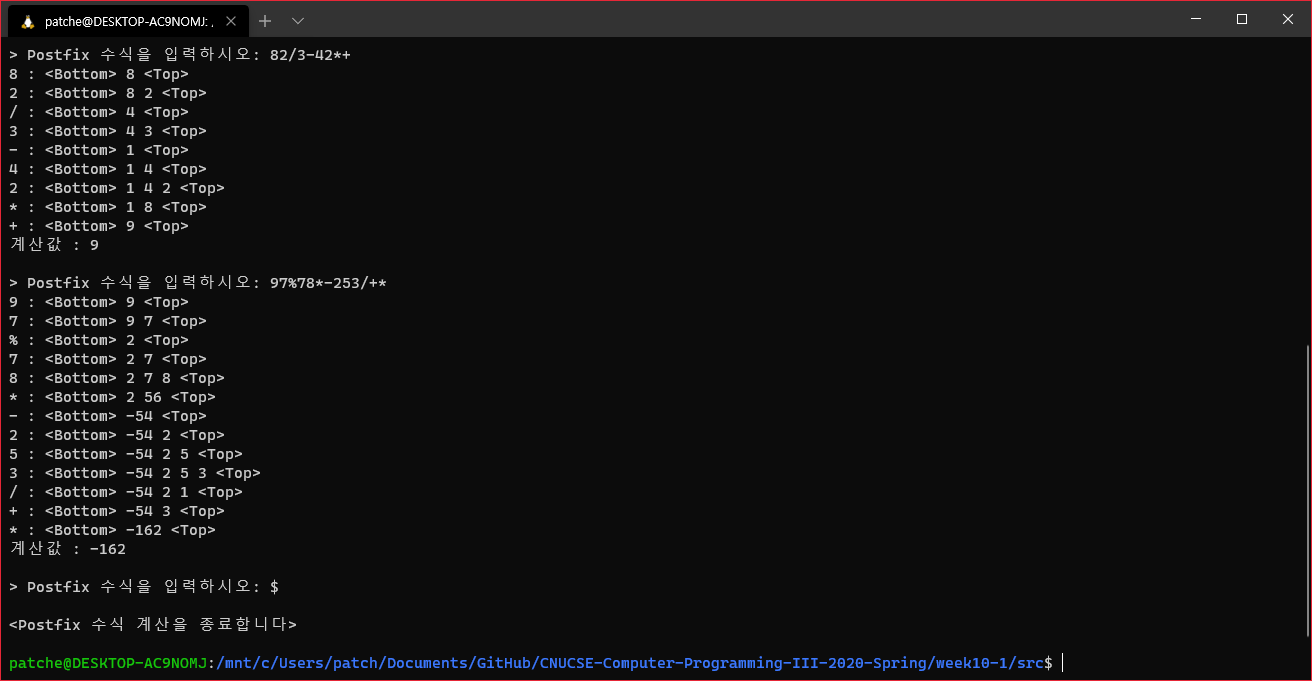
\includegraphics[width=\textwidth]{result_2.png}
                \caption{자료 제시 입력 실행결과 2}
                \label{}
            \end{figure}
        }

        \newpage

        \section{입력과 출력}
            실습 자료에서 제시된 입력을 사용하였으며 출력 결과는 상기한 것과 같았음.
        \section{결과 분석}
            모든 입력에 대하여 정상적인 출력을 확인하였음.

    \chapter{소스코드}
        소스코드는 제출된 압축파일에 같이 동봉되어있으며 GitHub (0x00000FF/CNUCSE-Computer-Programming-III-2020-Spring) 에서도 열람할 수 있다.
\end{document}